\documentclass[a4j]{jsarticle}

\usepackage{listings}
\usepackage{color}
\usepackage{ascmac, here, txfonts, txfonts}
\usepackage[dvipdfmx]{graphicx}
\usepackage{comment}
\usepackage{otf}

\lstset{
  basicstyle={\ttfamily},
  identifierstyle={\small},
  commentstyle={\smallitshape},
  keywordstyle={\small\bfseries},
  ndkeywordstyle={\small},
  stringstyle={\small\ttfamily},
  frame={tb},
  breaklines=true,
  columns=[l]{fullflexible},
  numbers=left,
  xrightmargin=0zw,
  xleftmargin=3zw,
  numberstyle={\scriptsize},
  stepnumber=1,
  numbersep=1zw,
  lineskip=-0.5ex
}

\renewcommand{\lstlistingname}{ソースコード}


\begin{document}

\begin{titlepage}
  \title{情報特別演習\ajRoman{2} 最終レポート\\ Kinectによる自然な姿勢推定の実現}
  \author{情報科学類2年\\堤海斗}
  \maketitle
  \thispagestyle{empty}
  
\end{titlepage}

\begin{comment}
  ・演習概要
    ・演習テーマと背景
    ・演習目的
  ・演習手法
    ・FKによる姿勢推定
    ・自然な姿勢推定
      ・IKの導入
      ・キャリブレーションの導入
      ・フィルターの導入
  ・演習結果とまとめ
    ・実装結果
    ・現在取り組んでいる項目
    ・今後の展望
    ・演習で得られたこと
\end{comment}

\section{演習概要}

\subsection{演習目的}

今年の情報特別演習\ajRoman{2}では、「Kinectによる自然な姿勢推定の実現」
というテーマで1年間演習をしてきた。
本演習の目的は、Kinect v2というデバイスを用いて人の動きをセンサリングし、
そのデータを人型アバターに反映するという一連のシステム、つまり
モーションキャプチャシステムの実装において、
より自然な姿勢推定を実現することを目的としている。

本演習では以下の環境を用いる

\begin{itemize}
  \item Kinect v2
  \item Unity 2018.4.xx 
\end{itemize}

\subsection{演習の背景}

前述のとおり本演習ではKinect v2というデバイスを使うのだが、
このデバイスはMicrosoftが開発していた赤外線カメラデバイスの1種である。
このデバイスではカラーカメラによって通常のカラー画像をはじめ、
赤外線による深度画像が取得可能である。
加えて深度画像を解析して人間を検知し、人の関節データを取得することが可能である。
Kinectだけでも姿勢推定は可能なのだが、
今回はUnityを用いてVRMやMMDといった人型アバターモデルに適用することで、
モーションキャプチャをしようと考えた。

このようなテーマにした理由として、昨今のVTuberブームが挙げられる。
2017年下旬から”VTuber”とよばれるコンテンツが話題になっていた。
VTuberとは人間の動きをモーションキャプチャによってバーチャルなキャラクターに反映し、
Youtubeなどの動画配信プラットフォームで動画投稿や配信活動をするコンテンツである。

私はこのVTuberにとても興味があり、
このようなものを自分でも実現してみたいと思い、このテーマを選択した。
Kinect v2は最初に今回演習で担当をして下さっている志築先生のIPLABからお借りして、
その後に、夏の長期休み明けからは自分の私物を使った。

\subsection{モーションキャプチャについて}

本演習ではモーションキャプチャシステムを作ることが目的であるので、
そもそもモーションキャプチャとは何かについて説明する。

前節で少し言及した通り、モーションキャプチャとは
人をはじめとしたものの動き(モーション)をセンサリングで取得する(キャプチャ)ことである。
モーションキャプチャを利用して、前述したVTuberやゲームキャラクターのモーション作成、
ジェスチャーインプットを使ったアプリケーションの作成などができる。

モーションキャプチャを行うには、モーションキャプチャができるデバイスが必要だが、
どの程度のモーションキャプチャが必要かどうかによって必要な機材が変わってくる。
例えば、上半身だけのモーショントラッキングであれば、
顔の位置と表情をトラキングできればよいのでスマホ1台でもできる。
そこに手の動きを加えたければLeapMotionなどのデバイスを使う。
また、立った姿でトラッキングをするとなると、VRセットが活用できる。
Oculus Questなどのデバイスを使うことによって
VRアプリケーションを操作するために最適なモーションキャプチャが可能である。

今回の演習では、全身を使った、いわゆるフルトラッキング・モーションキャプチャをする。
フルトラッキングができるデバイスの例を以下に示す。

\begin{itemize}
  \item VICON
  \item OptiTrack
  \item Vive Tracker
  \item Perception Nueron
  \item RealSense
  \item iPhone 11 Pro
\end{itemize}

精度の差はあれど、これらのデバイスをセンサーとして用いることで
モーションデータの取得が可能であり、
取得したデータを利用してアプリケーションを開発する。

本演習ではKinect v2を使ってモーションキャプチャをするわけだが、
前述のとおり、Kinect v2では、Kinect自身でモーションキャプチャが完結しており、
モーションデータをUnityやC++アプリケーションでリアルタイムに取得可能である。
Kinect v2の主な特徴は以下のとおりである。

\begin{itemize}
  \item 非接触型センサーである
  \item Unity用のSDKが配布されている
  \item 複数人のモーションキャプチャが同時にできる
  \item 開発が終了している
\end{itemize}

非接触型センサーとは、対象物にデバイスを接触させないでセンサリングする方法である。
通常、モーションキャプチャデバイスでは、トラッカーと呼ばれるデバイスを
関節に装着したりマーカーを全身に着けたりするのだが、
Kinectでは深度情報から姿勢推定をするため、そのような手間がない。
したがって他のデバイスと比べてユーザ・エクスペリエンスが高いという特徴がある。

また、Kinectは開発元のMicrosoftからUnity用のSDKが配布されており、
Unityのプロジェクトにインポートすることで容易に開発を始めることができる。
UnityではScene内にプレハブ展開し、ゲームオブジェクトにスクリプトをアタッチすることで
UnityのAPIを利用したプログラムを実行できるのだが、
ポーリング式でセンサーデータを取得する場合には
プレハブもスクリプトも用意してある。

しかし、Kinect v2はサポートが終了しており、
開発が進められていないというデメリットがある。
実際、Kinectの用途として、深度情報から点群情報を解析して利用することが多く、
BodyTrackingに関しては文献が少ないというデメリットもある。

\section{演習手法}

\subsection{FKによる姿勢推定}

モーションキャプチャを行うにあたって、まず初めにFKという手法を用いて
アバターのボーンを制御した。
FKは"Forward Kinematics"の略で、日本語訳すると"順運動学"ということになる。
順運動学とはボーン制御手法の1種で、
目的の姿勢を親のボーンデータから推定していく手法を指す。

例えば、人間の腕のような2ボーンFKを考えると、
まず肩のボーンの回転を取得する。そして肩のボーンを親に持つ肘のボーン
の位置が決まる。
そして肘の回転から手首の位置が決まる、という風にボーンを推定・制御していく。

FKはとても直観的なロジックなため実装自体は簡単だが、
センサリングを行う上で生じる誤差が末端のボーンに行くにつれ蓄積されていくという
致命的な欠点がある。
また、FKでは推定するすべての関節データが必要になってくるため、
広く使われているようなトラッカーを使うモーションキャプチャには適用するのが難しい。

実際に、Kinectのモーションデータ(回転データ)をそのまま適用してみた結果、
以下の画像のようになってしまった。

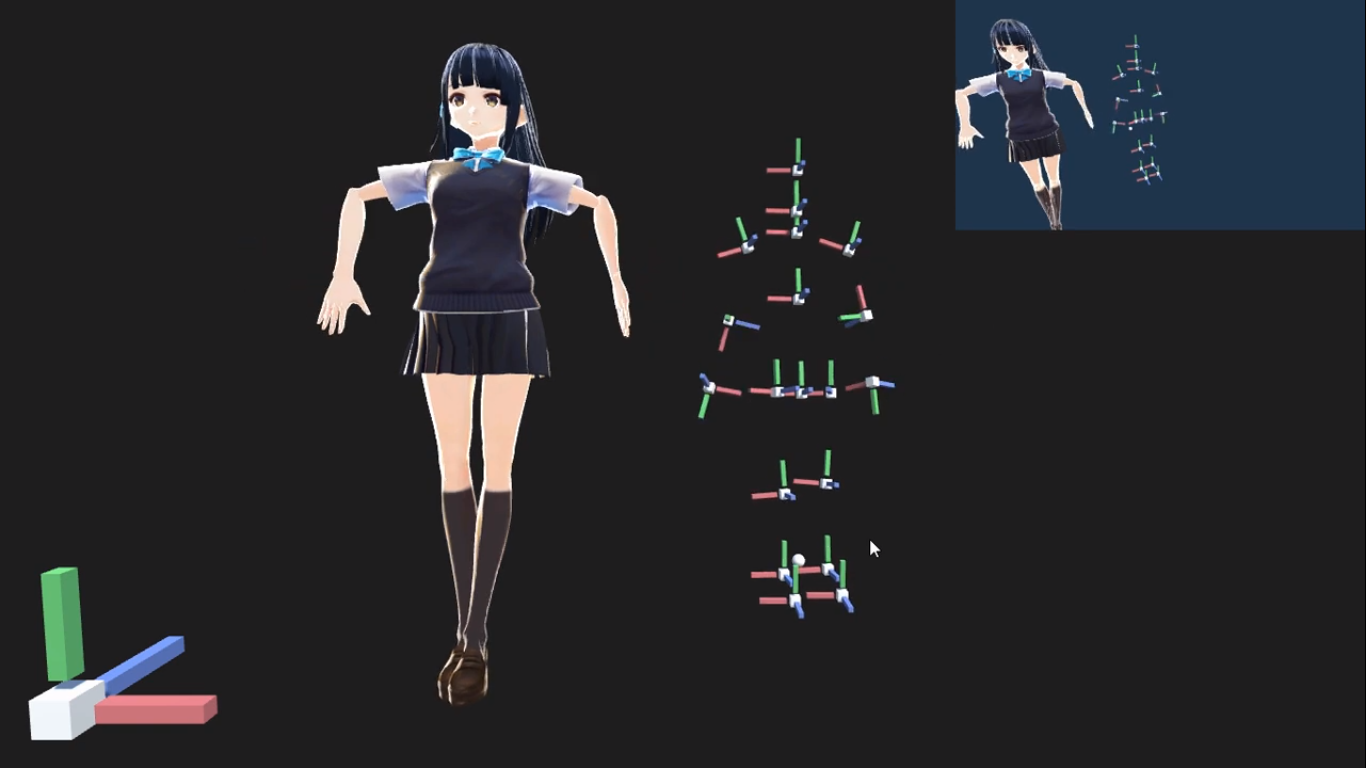
\includegraphics[width=10cm]{img/fk-noise}

これは肩のボーンの回転が適当に取得できなかったため、
それが肘、手首のデータの誤差と共に蓄積されてしまった結果である。
本来ならば気を付けの姿勢をしているが、肩が回転しなかったため、
肘が横に行ってしまっている。


\subsection{自然な姿勢推定}

前節のように、FKだけだとうまくボーンデータを反映することができなかった。
ここでは本演習の主題でもある「自然な姿勢推定」を実現するために導入した手法を説明していく。

\subsubsection{IKの導入}

FKでは、一番親のボーンから末端のボーンまでを推定していたが、
IKはその逆で、末端のボーンからその他のボーンデータを推定していく手法で、
"Inverse Kinematics"の略である。逆運動学とも言う。

IKを使うことにより、FKにおける問題を解消することができる。
FKでは末端のボーンに行くにつれ誤差が蓄積するという問題があったが、
IKは末端のボーンのデータによって他のボーンデータを推定するため、
誤差はボーンデータ1つ分で済む。
また、末端のボーンデータをとるためのトラッカーがあればよいので、
機材の観点からも利用の幅が広がるのである。

しかしFKよりもIKの実装には3次元の幾何学的な処理が必要になるため
実装は難易度が高くなり、計算量も多くなる。
そこで今回はUnityのMecanimというシステムを利用した。
Mecanimは、Unityで標準的に実装されているアバター制御のためのAPIで、
モデルがHumanoidとしてリギングされており、適切なAnimationControllerが設定されていれば、
IKに必要な末端のボーンの位置/回転、適用する重さを設定することにより
容易にIK制御を実現できる。


\subsubsection{キャリブレーションの導入}

IKを導入すると、必然的に回転の他に位置の概念が重要になってくる。
モーションキャプチャのターゲットとなる人間と
モーションデータを反映するアバターとの位置合わせを行う必要がある。
そこでキャリブレーションとレジストレーションという二つの処理を導入する。

キャリブレーションとは本格的なセンサリングをする前に、
センサーの標準状態を測定することを言う。
モーションキャプチャでのキャリブレーションは、
ターゲットとなる人間のボーンデータをあらかじめ測定し、
体格を把握することを指す。

モーションキャプチャをするときにモーションデータを反映する際に
体格の違いによって、例えば腕の長さが違うことにより
ターゲットの人間は腕を伸ばしているのに、
アバターは腕が伸び切っていないような状態になることがある。
それを解決するためにまず人間の体形を把握し、
キャリブレーションした体形から、相対的にアバターの関節の位置を割り出す必要がある。
相対的なボーンデータを割り出し、アバターに反映する操作をレジストレーションと呼ぶ。

\subsubsection{フィルターの導入}

\section{演習結果とまとめ}

\subsection{実装結果}

\subsection{現在取り組んでいる項目}

\subsection{今後の展望}

\subsection{本演習で学んだこと}


\end{document}